\documentclass{article}
\usepackage[utf8]{inputenc}
\usepackage{amssymb}
\usepackage{amsmath}
\usepackage{float}
\usepackage{epstopdf}
\usepackage{moreverb}
\usepackage{multicol}
\usepackage{listings}
\usepackage{mathrsfs}
\usepackage{graphicx}
\usepackage{cite}
\usepackage{tabularx}
\usepackage{listings}
\usepackage{subcaption}
\newcommand{\R}{\mathbb{R}}
\newcommand{\overbar}[1]{\mkern 1.5mu\overline{\mkern-1.5mu#1\mkern-1.5mu}\mkern 1.5mu}


\bibliographystyle{plain}
\title{APPM 5720 Homework 4}
\author{Wil Boshell, Fortino Garcia, Alex Rybchuk, Parth Thakkar}
\date{February 22, 2018}


\begin{document}

\maketitle

\maketitle

\noindent The main task of this homework is to approximate the transport equation
	\begin{align*}
		u_t + \left( a u\right)_x = 0, \quad x_L \leq x \leq x_R, \quad t > 0,
	\end{align*}
with initial conditions $u(x,0) = f(x)$.
\subsection{Approximate $\left( a u\right)_x $ on a single element with no boundary conditions}
Lut $u$ be a function approximated on $x_L \leq x \leq x_R$, by a polynomial of the form
	\begin{align*}
			u(x(r)) \approx u^h \equiv \sum_{k=0}^q \hat{u}_kP_k(r).
	\end{align*}
If $a$ is constant, we seek another polynomial $b(x)$
	\begin{align*}
		b(x) = \sum_{k=0}^q \hat{b}_kP_k(r),
	\end{align*}
such taht the coefficients $\hat{b}_k$ solve the linear system of equations

	\begin{align*}	
		\int_{x_L}^{x_R}bP_l\, dx = \int_{x_L}^{x_R} P_l \frac{d(au^h)}{x} dx, \, \quad l = 0,\dots,q.
	\end{align*}	
Pluggin in our previous expression, we arrive at 
	\begin{align*}	
		\int_{x_L}^{x_R}bP_l\, dx = a \sum_{k=0}^q \int_{x_L}^{x_R} P_l P_k' dx, \, \quad l = 0,\dots,q.
	\end{align*}
This leads to a matrix system of the form
	\begin{align*}
		M \boldsymbol{\hat{b}} = a S \boldsymbol{\hat{u}},
	\end{align*}
where the matrix $M$ is a diagonal matrix as in the previous homework. This scheme is implemented for the following functions
	\begin{align*}
		f(x) = e^x + \cos x, \quad g(x) = e^{-x^2}, \quad h(x) = x^8.
	\end{align*}
The error plots for increasing $q$ are below.

\begin{figure}[H]
  \centering
  \begin{minipage}{.4\textwidth}
    \centering
    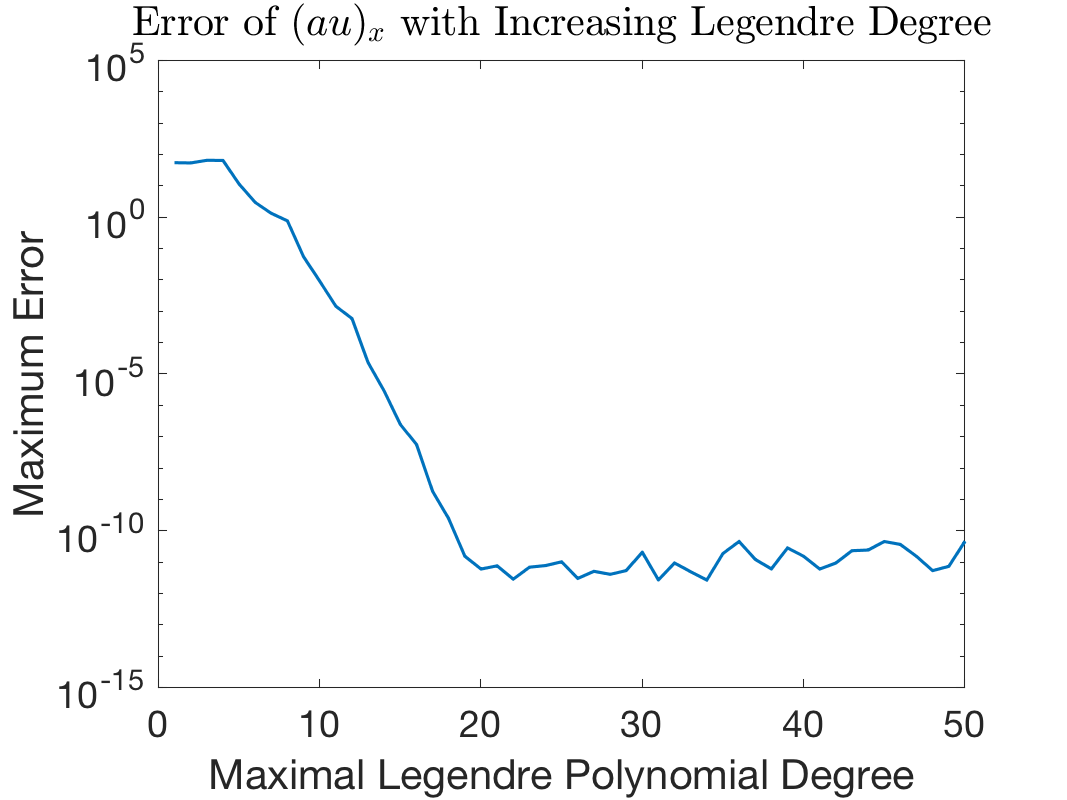
\includegraphics[width=\linewidth]{plots/exp_cos.png}
    \captionof{figure}{$f(x)$}
    \label{fig:max0}
  \end{minipage}%
  \begin{minipage}{.4\textwidth}
    \centering
    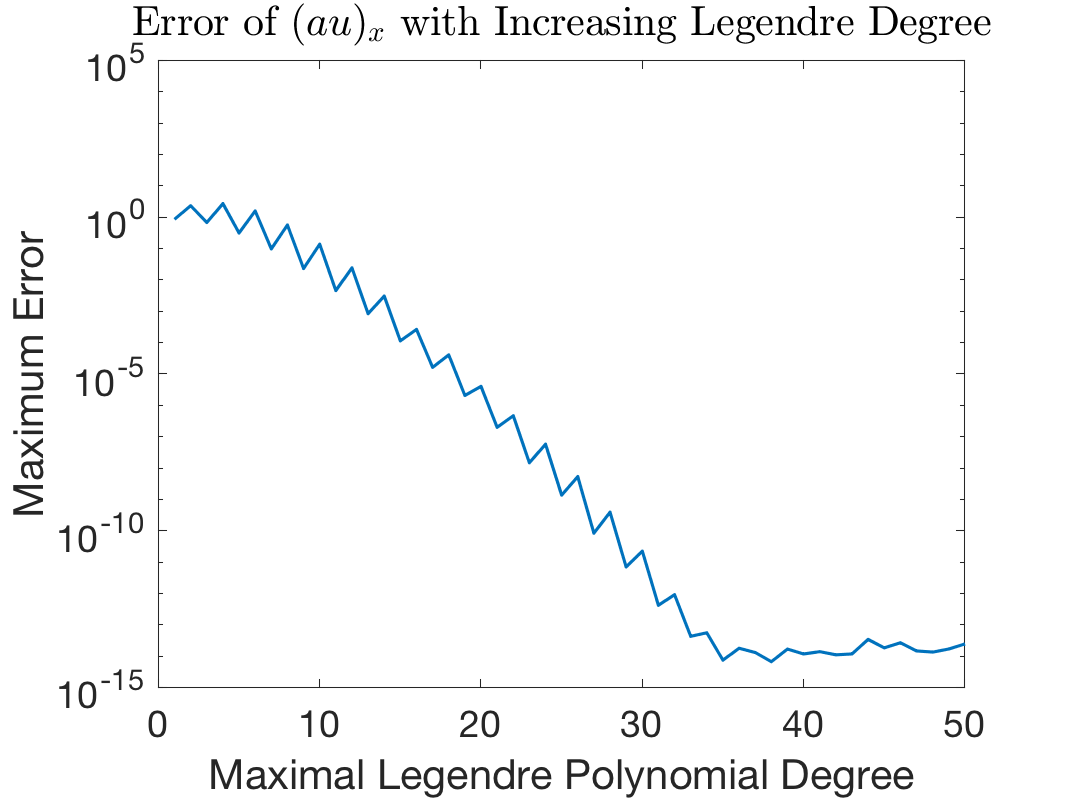
\includegraphics[width=\linewidth]{plots/gaussian.png}
    \captionof{figure}{$g(x)$}
    \label{fig:square0}
  \end{minipage}%
  \begin{minipage}{.4\textwidth}
    \centering
    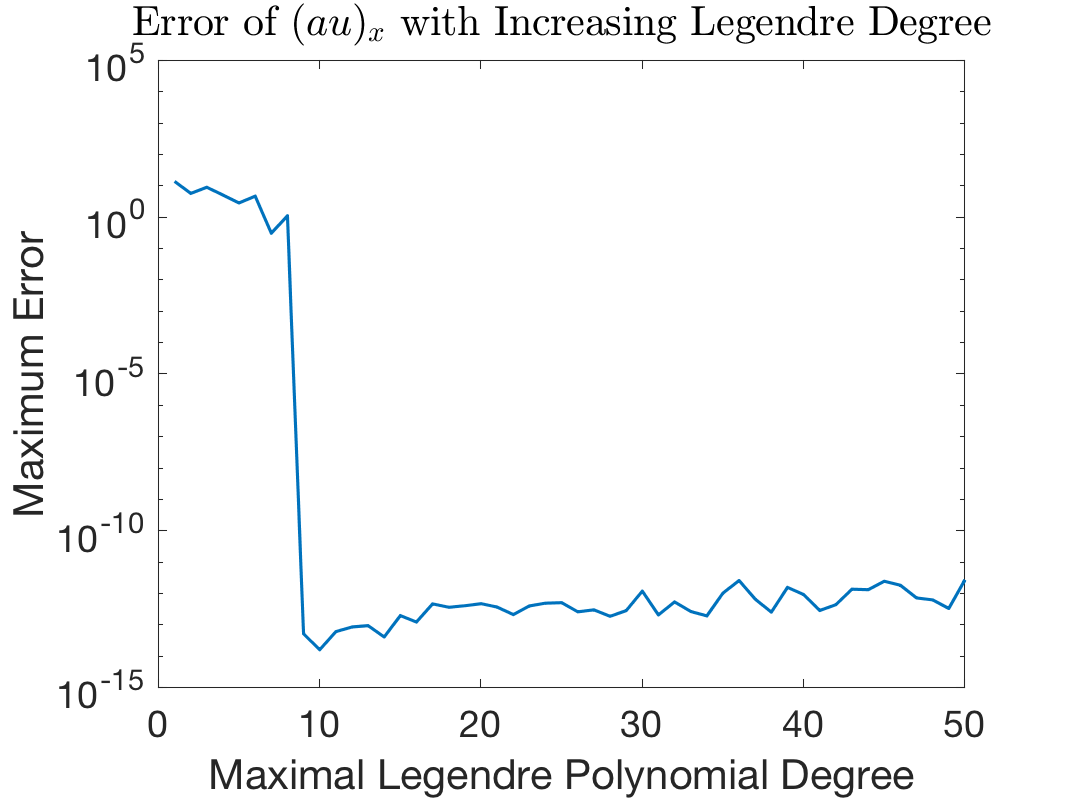
\includegraphics[width=\linewidth]{plots/x_8.png}
    \captionof{figure}{$h(x)$}
    \label{fig:eight}
  \end{minipage}%
\end{figure}
\noindent From these plots it is clear that with increasing $q$ the error decreases until roundoff error takes over soon after achieving $11-12$ digits of accuracy. Curiously, the error plot for the Gaussian increases sharply depending on the even/oddness of $q$.

\subsection{Approximate $\left( a u\right)_x $ on a single element with boundary conditions}
Here we assume that $a(x)$ is \textbf{not} constant. We may integrate by parts to arrive at a system of equations of the form
	\begin{align*}
		M \boldsymbol{\hat{b}} = -S^a \boldsymbol{\hat{u}} + a(x_R)u^h(x_R)\boldsymbol{L_R} - a(x_L)u^h(x_L)\boldsymbol{L_L},
	\end{align*}
for which we solve for the spatial derivative coefficients $\boldsymbol{\hat{b}}$. We consider the case 
	\begin{align*}
		& a(x) = \frac{2}{2 + \sin x} \quad -\pi \leq x \leq \pi \\
		& u(x) = \exp(\sin x) \quad -\pi \leq x \leq \pi.
	\end{align*}
We note that the exact spatial derivative of the product is 
	\begin{align*}
		(a(x)u(x))_x = \frac{2 \exp(\sin x) (\sin x + 1) \cos x}{(\sin x + 2)^2},
	\end{align*}
which we use to compare our computed solution against. Below is a plot of the error with increasing degree of Legendre polynomial.

\begin{figure}[H]
  \centering
  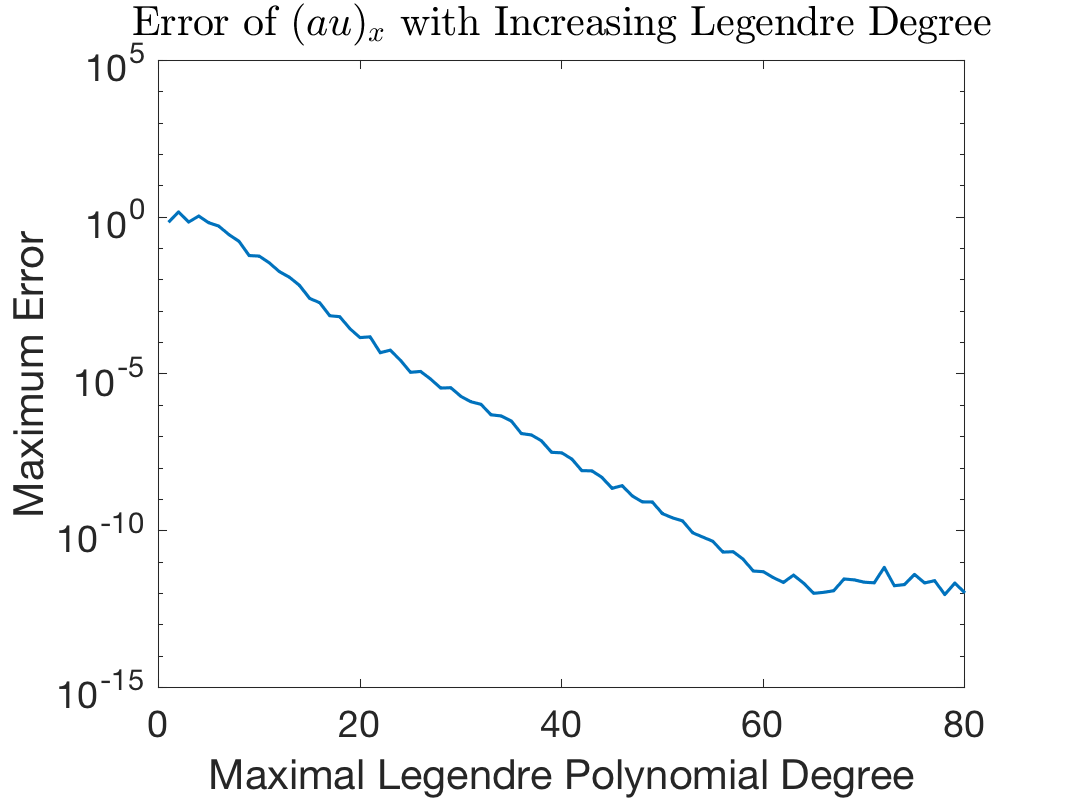
\includegraphics[scale=0.5]{plots/var_coeff.png}
  \caption{Plot of Increasing Legendre degree $q$ for Spatial Derivative Computation}
  \label{fig:spatDer}
\end{figure}
\noindent As before, we notice that we get steadily decreasing error until we achieve aroun $11-12$ digits of accuracy, after which roundoff errors steadily increase the error in the computation of the derivative. To further understand this process, we compute the eigenvalues of the matrix $A$, defined through $\boldsymbol{\hat{b}} = A \boldsymbol{\hat{u}}$. We assume periodic boundary conditions and a constant coefficient $a = 1$ for the following plots, which were generated by calling \verb|dgeev| and ploting via MATLAB. First let us examine the behavior of $\lambda _{max}$ with respect to increasing $q$ (and here we normalize by the scaling factor in the affine map):

\begin{figure}[H]
  \centering
  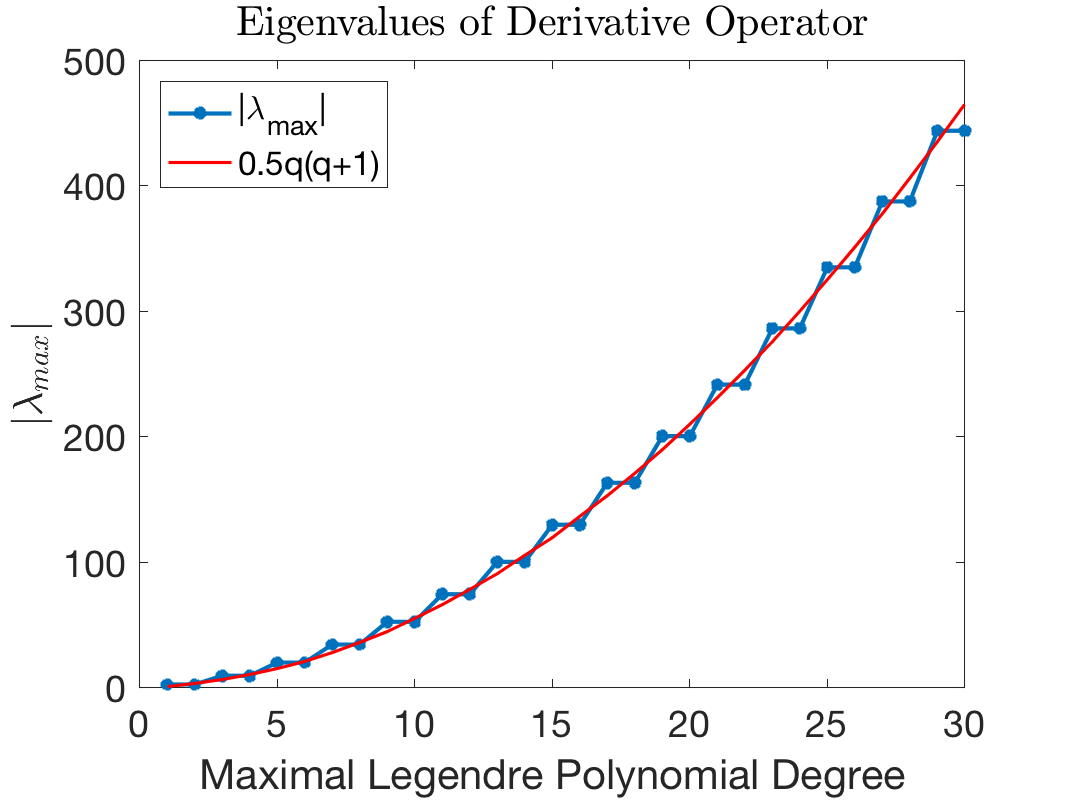
\includegraphics[scale=0.7]{plots/eig_data.png}
  \caption{Plot of $\lambda _{max}$ with Increasing $q$}
  \label{fig:eig_data}
\end{figure}

\noindent Recalling that 
	\begin{align*}
		P_n'(1) = \frac{n(n+1)}{2}, 
	\end{align*}
we notice that the maximum eigenvalues of our matrix grow like $O(q^2)$ while the "size" of $e^{iqx}$ is $q$. Then in a sense, our matrix creates functions which are "larger" than their true derivative. We plot some of the eigenvalues of the matrix for various values of $q$ in the complex plane:

\begin{figure}[H]
  \centering
  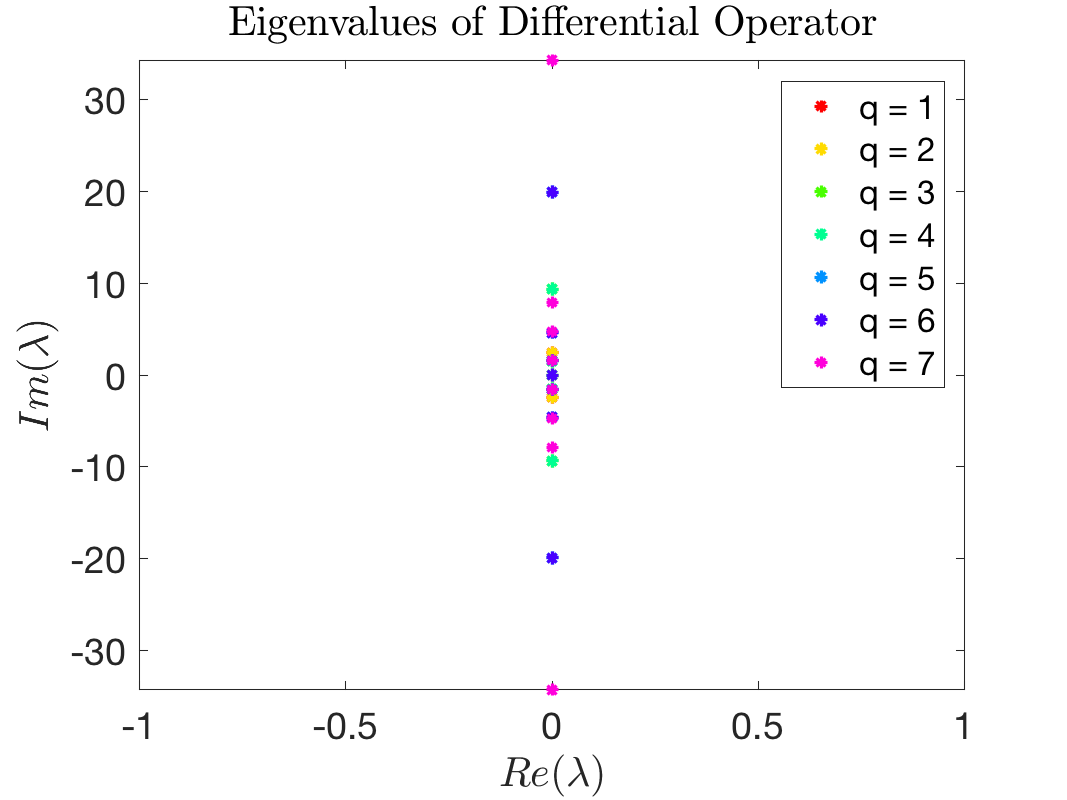
\includegraphics[scale=0.7]{plots/eig_plot.png}
  \caption{Plot of $\lambda$ for various $q$}
  \label{fig:eig_values}
\end{figure}
\noindent Indeed, the eigenvalues grow as $q$ increases as indicated by the previous plot. We note additionally that the eigenvalues are purely imaginary. Since the matrix has real entries, the characteristic polynomial has real coefficients and so the roots of this polynomial (the eigenvalues of $A$) appear in complex conjugate pairs. As a result, even powers of $q$ (which create matrices of odd size) must have a $0$ eigenvalue. Intuitively, these matrixes must always have an eigenvalue of $0$ since they represent a differential operator which is not invertible.

\subsection{Approximate $u_t + \left( a u\right)_x = 0$ on a single element with periodic boundary conditions}
For this task, we let $a$ be constant. As in the previous scheme, we have a matrix system of the form
	\begin{align*}
		M \boldsymbol{\hat{u'}}(t) = -S^a \boldsymbol{\hat{u}} + a(x_R)u^h(x_R)\boldsymbol{L_R} - a(x_L)u^h(x_L)\boldsymbol{L_L},
	\end{align*}
We use the code from last week's assignment to project the intial data to the space of Legendre polynomials, solve this system for the coefficients $\boldsymbol{\hat{u'}}(t)$, and use RK4 to time step and evolve our solution. For this problem we consider the following:

	\begin{align*}
		u_t + \left( a u\right)_x & = 0, \quad -\pi \leq x \leq \pi \\
		u(x,0) & = \cos x,
	\end{align*}
with explicit solution $u(x,t) = \cos (x - t)$. A "movie" (gif) of the result can be found on the main page of our repository for this homework as part of the README file. Below is a plot of the $L_2$ error of the computed solution as time evolves for various $q$ and step sizes $\Delta t$.

\begin{figure}[H]
  \centering
  \begin{minipage}{.4\textwidth}
    \centering
    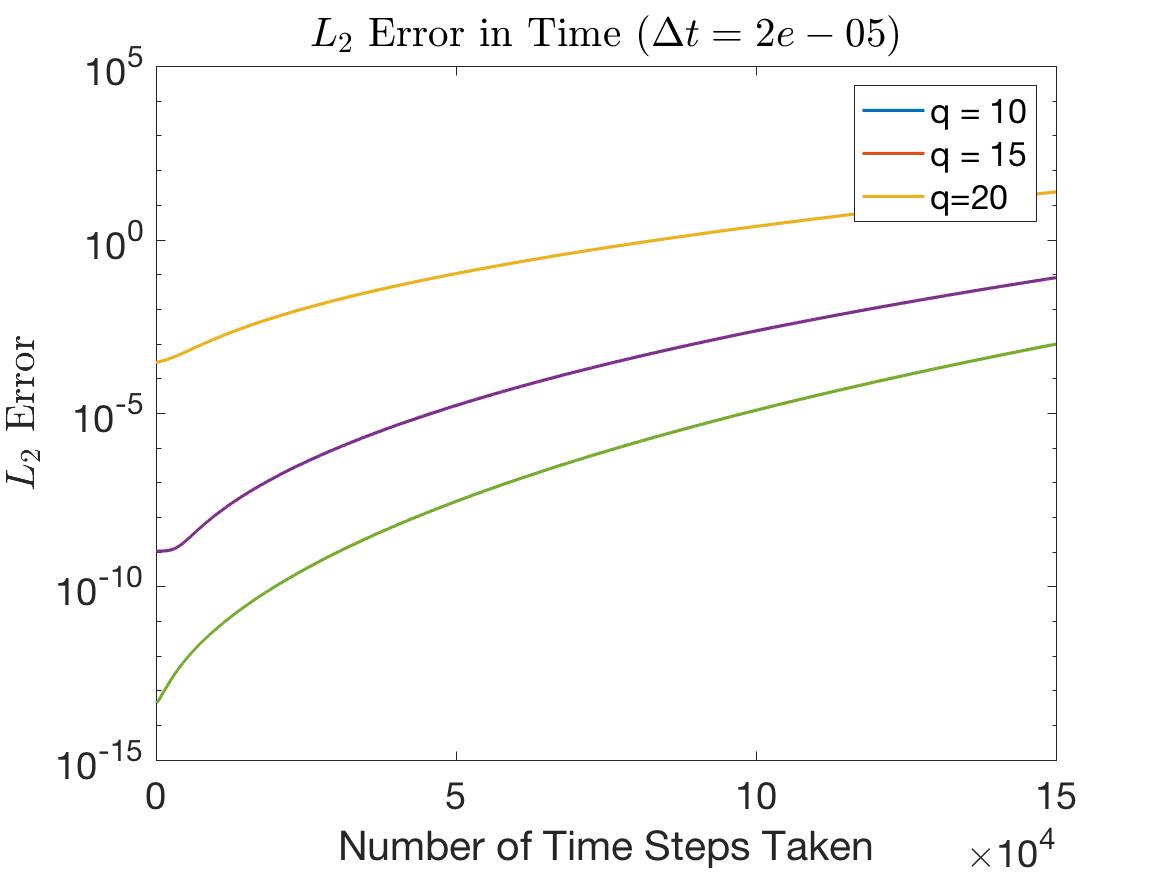
\includegraphics[width=\linewidth]{plots/l2_time_1.png}
    \label{fig:smallstep}
  \end{minipage}%
  \begin{minipage}{.4\textwidth}
    \centering
    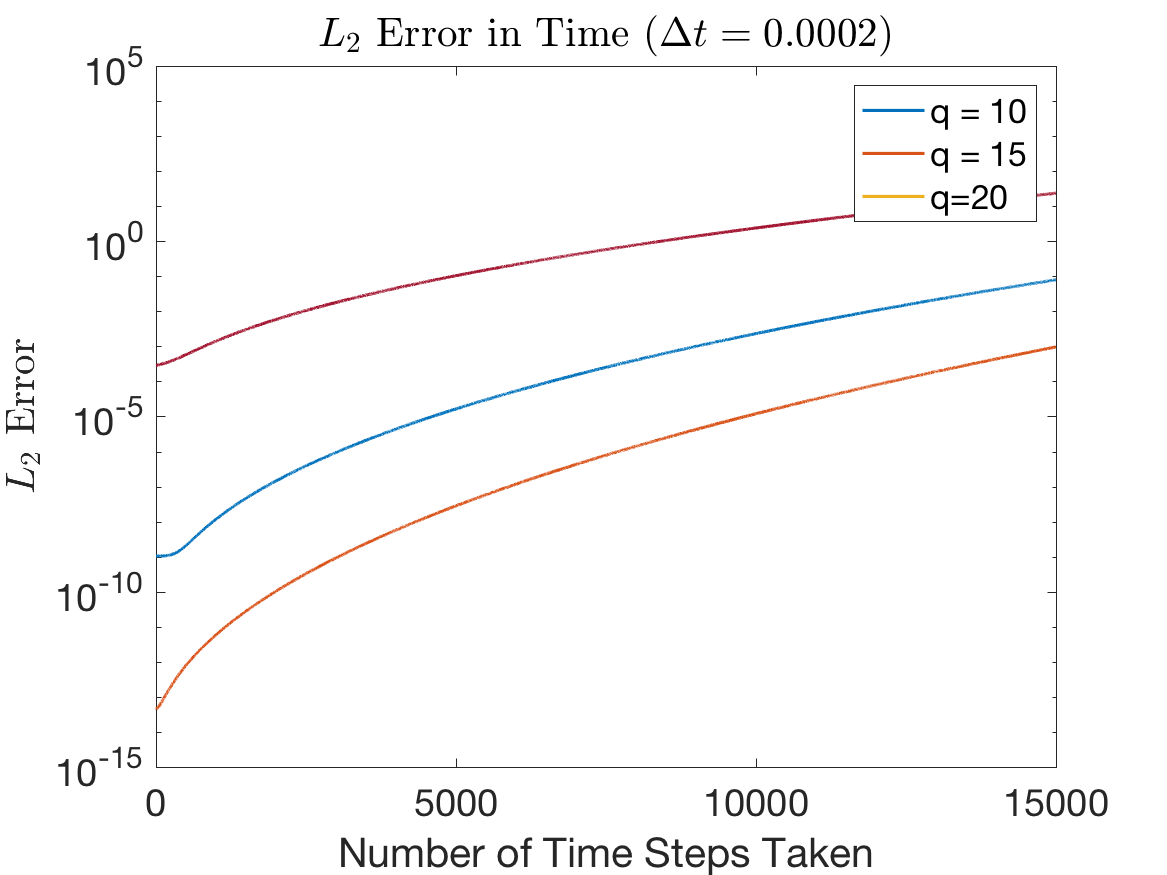
\includegraphics[width=\linewidth]{plots/l2_time_2.png}
    \label{fig:medstep}
  \end{minipage}%
  \begin{minipage}{.4\textwidth}
    \centering
    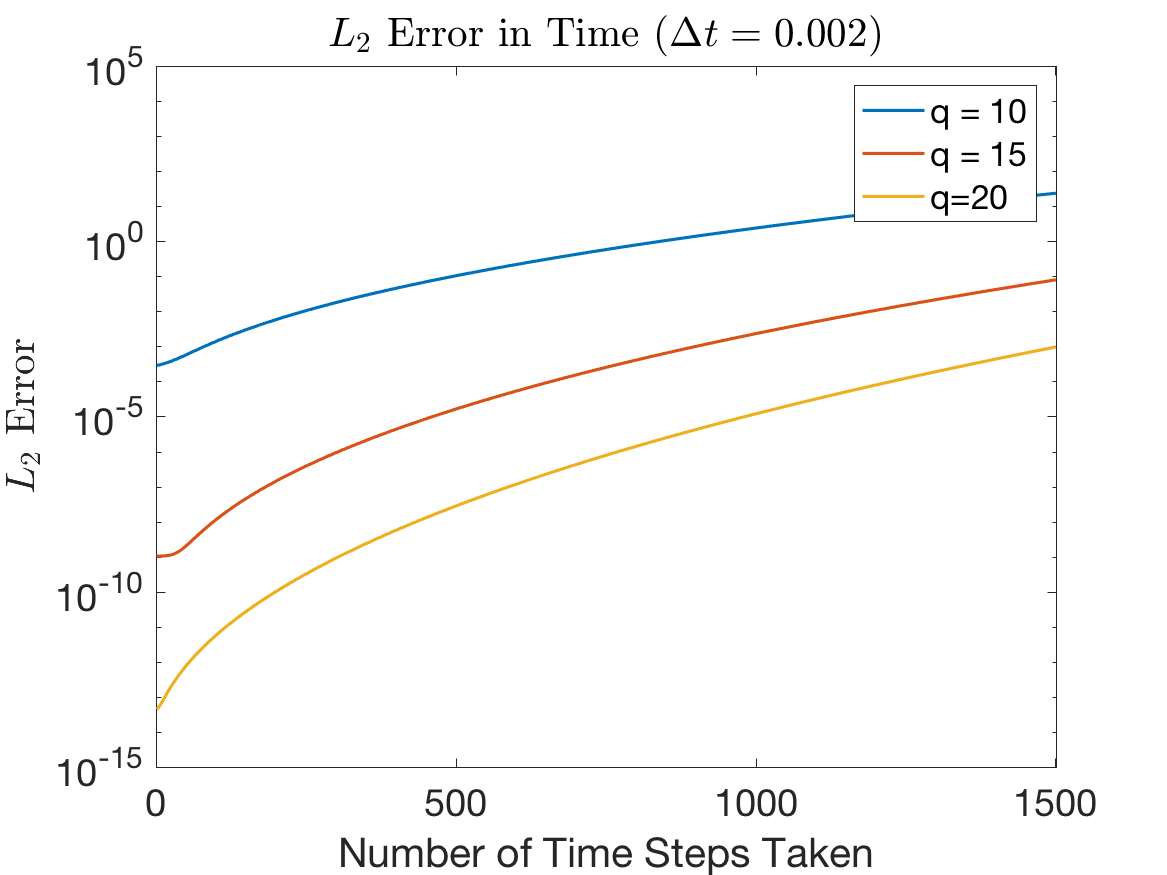
\includegraphics[width=\linewidth]{plots/l2_time_3.png}
    \label{fig:bigstep}
  \end{minipage}%
\end{figure}
\noindent We note that increasing $q$ leads to much better error estimates, but with a large enough number of time steps we lose accuracy and the errors grow in time.

\subsection{Approximate $u_t + \left( a u\right)_x = 0$ on a grid with inter-element and physical conditions}
We bring the previous results together and implement a discountinuous Galerkin solver for the test problem
	\begin{align*}
		u_t + \left( a u\right)_x & = 0, \quad -\pi \leq x \leq \pi \\
		u(x,0) & = \sin x,
	\end{align*}
with explicit solution $\sin (x-t)$. Below are various plots for different values of $\beta$. Note that the plots are such that red corresponds to the smallest value of $q$ and violet is the largest (i.e. $q$ is ordered according to ROYGBV). Running the script \verb|FinalPlot.p| generates this data and plots with MATLAB.

\begin{figure}[H]
  \centering
  \begin{minipage}{.4\textwidth}
    \centering
    \includegraphics[width=\linewidth]{plots/finalplot_1.png}
  	\caption{$\beta = 0$}
    \label{fig:beta0}
  \end{minipage}%
  \begin{minipage}{.4\textwidth}
    \centering
    \includegraphics[width=\linewidth]{plots/finalplot_2.png}
  	\caption{$\beta = 0.5$}
    \label{fig:beta1}
  \end{minipage}%
  \begin{minipage}{.4\textwidth}
    \centering
    \includegraphics[width=\linewidth]{plots/finalplot_3.png}
  	\caption{$\beta = 1$}
    \label{fig:beta2}
  \end{minipage}%
\end{figure}

\noindent Again, increasing $q$ leads to better overall errors but errors in time stepping accumulate and cause a loss of accuracy. 

\end{document}


